\chapter {MOTION SYNTHESIS FRAMEWORK}
\label{chap:msf}
\ifpdf
    \graphicspath{{CombineFramework/CombineFrameworkFigs/PNG/}{CombineFramework/CombineFrameworkFigs/PDF/}{CombineFramework/CombineFrameworkFigs/}}
\else
    \graphicspath{{CombineFramework/CombineFrameworkFigs/EPS/}{CombineFramework/CombineFrameworkFigs/}}
\fi

Chapter 3 and Chapter Discussion some important idea of natural motion control properties from the mechanical viewpoint.
In this chapter ,we will dicuss how we combine the idea from Chapter 3 and Chapter 5 into meaning full motion synthesis System.
Mainly we will discuss two question,
\begin{itemize}
\item how global and local motor invariant controller work together.
\item how combine different motion primitives together.
\end{itemize}

\section{Combined Global and Local Motor Invariant}

\subsection{ motor control idea based on Global and Local  Motor Invariant.}

Neural Oscillator will maintain the qualitative motion properties, and Controller Symmetry will satisfy the quantitative properties.
Basically we need apply the qualitative controller first to maintain the topology against the structural perturbation, 
when Symmetry Controller is applied to transform the entrainment System to meet some specific user constraints.


Snimply put, we should get the qualitative write first, and then get the quantitative write .
This idea is straightforward is illustrated in the following example
\begin{figure}[!htbp]
  \begin{center}
    \leavevmode
    \ifpdf
      \includegraphics[height=6in]{LimitCircle}
    \else
      \includegraphics[width=0.7\textwidth]{LimitCircle}
    \fi
    \caption{System Over View }
    \label{fig:sysoverview}
  \end{center}
\end{figure}
but when applying this method, we have condition must be met.
\begin{itemize}
\item unlike the CPG controlled example discussed in Chapter 3, when must maintain the topology when the symmetry controlled is applied.
To met this condition, we must prove that Symmetry Controller will not violate the topology, and symmetry control is applied to the how system rather than the original system.

We must prove that Lie Group Operator will not violate the topology

\item In chapter 4 we discuss the controlled symmetry is applied to the original system, how ever, for motion synthesis, we must prove that the combined system should preserve the symmetry.

If the original system $F(x)$ have the symmetry property, we also require the neural oscillator have the same symmetry properties.
Thus we need to discuss how to transform the Neural Oscillator so the neural oscillator have the same kind of symmetry as the mechanical oscillator
\end{itemize}



\subsection{ Controlled Symmetry Preserved The Topology}

Theorem Controlled Symmetry is Topology Preserving
suppose the original system is $\dot{x}=F(x)$, Controlled system is $\dot{G(x)}=F(G(x))$,
proof :
	by the demotion mation, G is continues and one one mapping.
	The the the original system and transformed system are isotropy.
	Thus Controlled Symmetry is topology Preserving


\subsection{ Symmetry of Neural Oscillator.}
We separate the discussion

after coupling with neural oscillator, the $\dot{x}=F(x)$ becomes a system 
$\dot{x}=F(x)+u_in$
for controlled system, when must maintain
$\dot{G(x)}=F(G(x)+u_ing$

for the neural system
the the dynamic equation is

$\dot{xc}=S(x_c)+uin$
we requires te symmetry must meet
$\dot{G(xc)}=S(G(x_c)+u_ing$
the out put function is
$O(x_c)$


for the symmetry property, we must statisfy the following following follow equation
$u_inG=O(x_cG)$
$u_inG=O(xg)$

For must our research, we find that we only adjust the three parameters of the neural oscillator to meet equation above
$\tau,hi,ho$
and some examples are included.

\subsubsection*{ offset Symmetry.}
For offset symmetry, we carefully select the $U_in$ and $U_out$ acting on the Invariant variables.
For example ,when walking slope changes, we choose the input of the neural oscillator to be the angle between the joints or velocity difference,
then all the input function will not change, if the output of the neural oscillator is apply not directly the q, but to the difference of q of velocity of q,
then the out put function can is also unchanged.


\subsubsection*{Time Scaling}
Neural Oscillator can change its Speed by changing ts.
We prove change ts, we can maintain the same is maintained.

For the dynamic system, usually control will affect the second order derivative.
Then we can u needs to be $ts^2$ the original system.
So we can multiply $hout=ts^2$ hout

\subsubsection*{ Energy Scaling}
energy scaling is $G(x)=(G(q),G(\dot{q})$
$q=sq$,
$\dot{q}=t(s)q$

it is equal to apply the scaling of the configure q and time scaling sequentially.
For our research, we apply the speed action to the neural oscillator first,
when scaling the h to keep the input keep constant.


\subsubsection*{time offset }
Neural Oscillator don't have to do any thing with the state,
but it also have to rotate its state.


\subsection{A simple example}

Bouncing Ball

\begin{figure}[!htbp]
  \begin{center}
    \leavevmode
    \ifpdf
      \includegraphics[height=6in]{BouncingBallPhasePlotAction1}
    \else
      \includegraphics[width=0.7\textwidth]{BouncingBallPhasePlotAction1}
    \fi
    \caption{Energy Scalling}
    \label{fig:energy1}
  \end{center}
\end{figure} 


\begin{figure}[!htbp]
  \begin{center}
    \leavevmode
    \ifpdf
      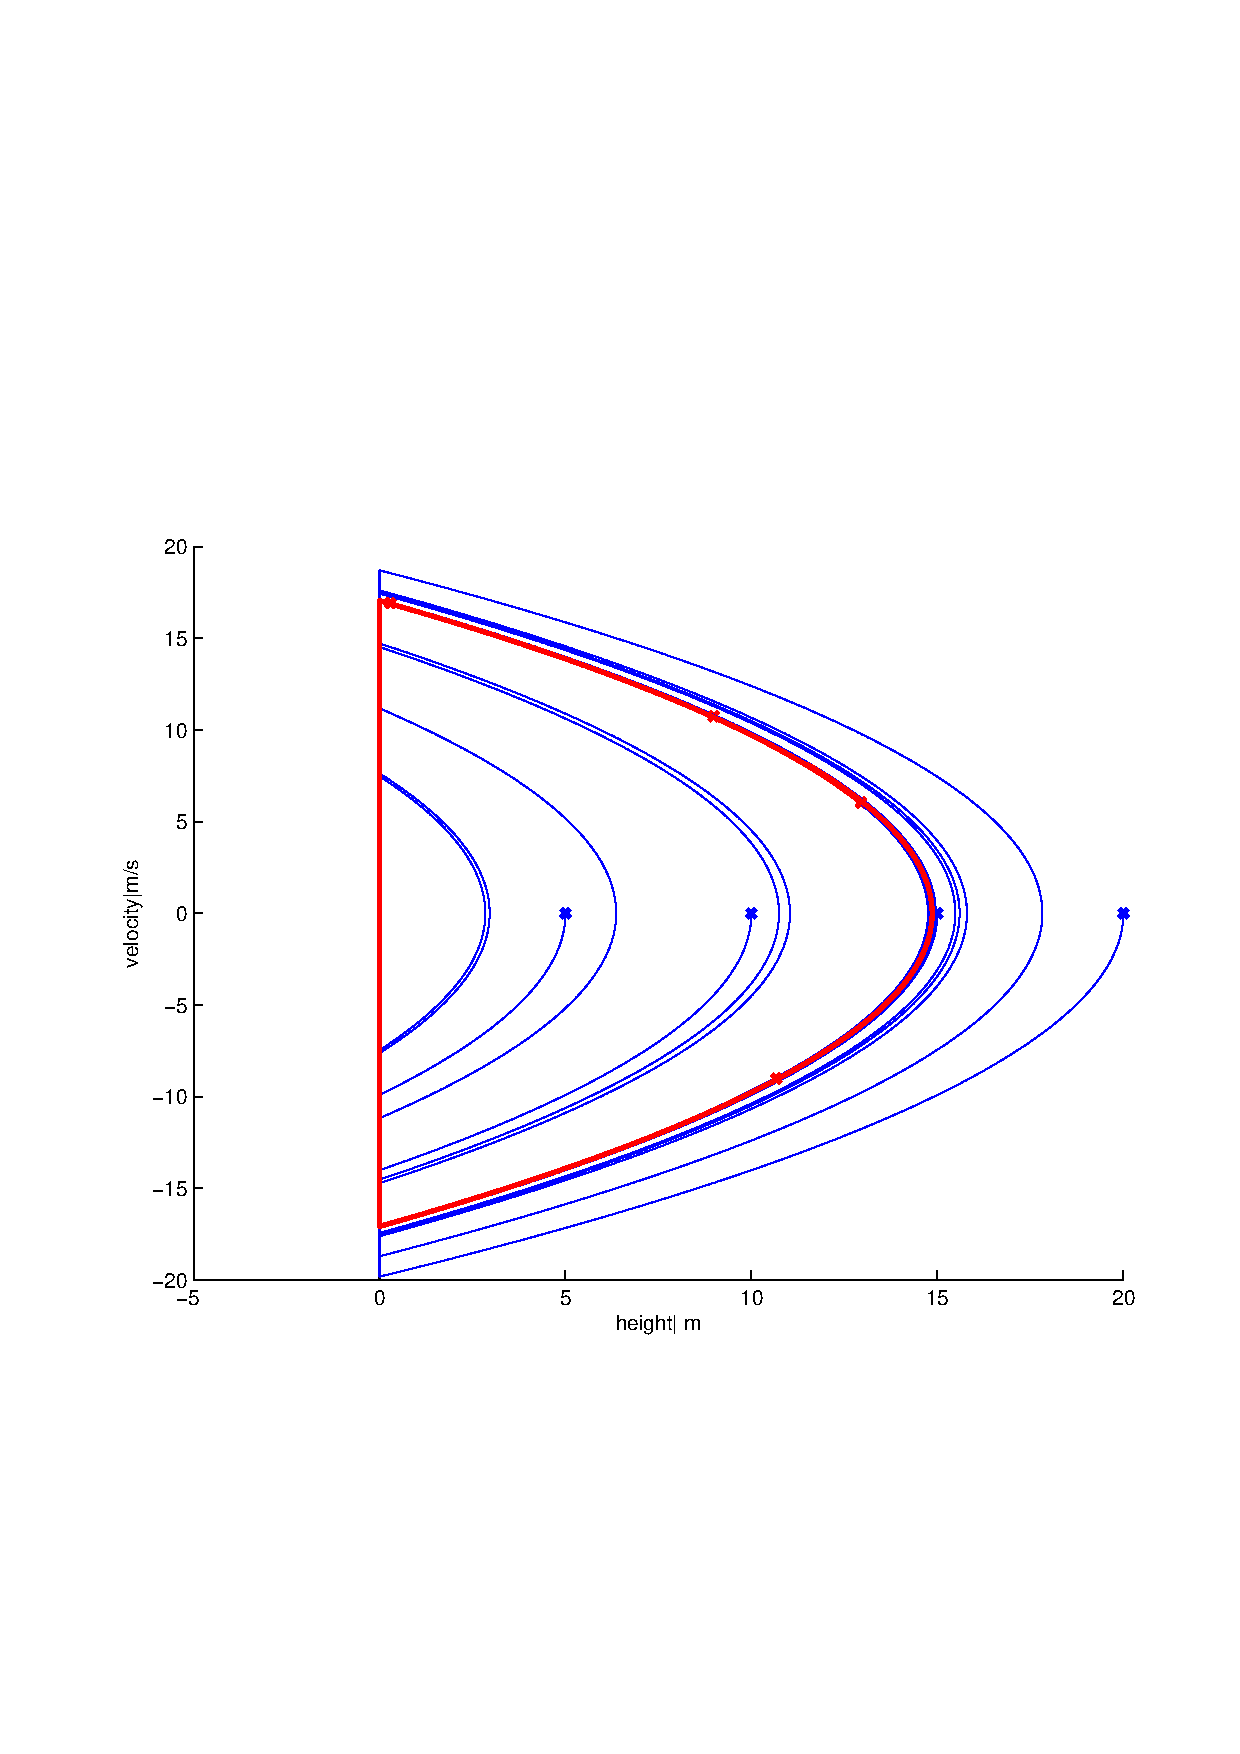
\includegraphics[height=6in]{BouncingBallPhasePlotAction3}
    \else
      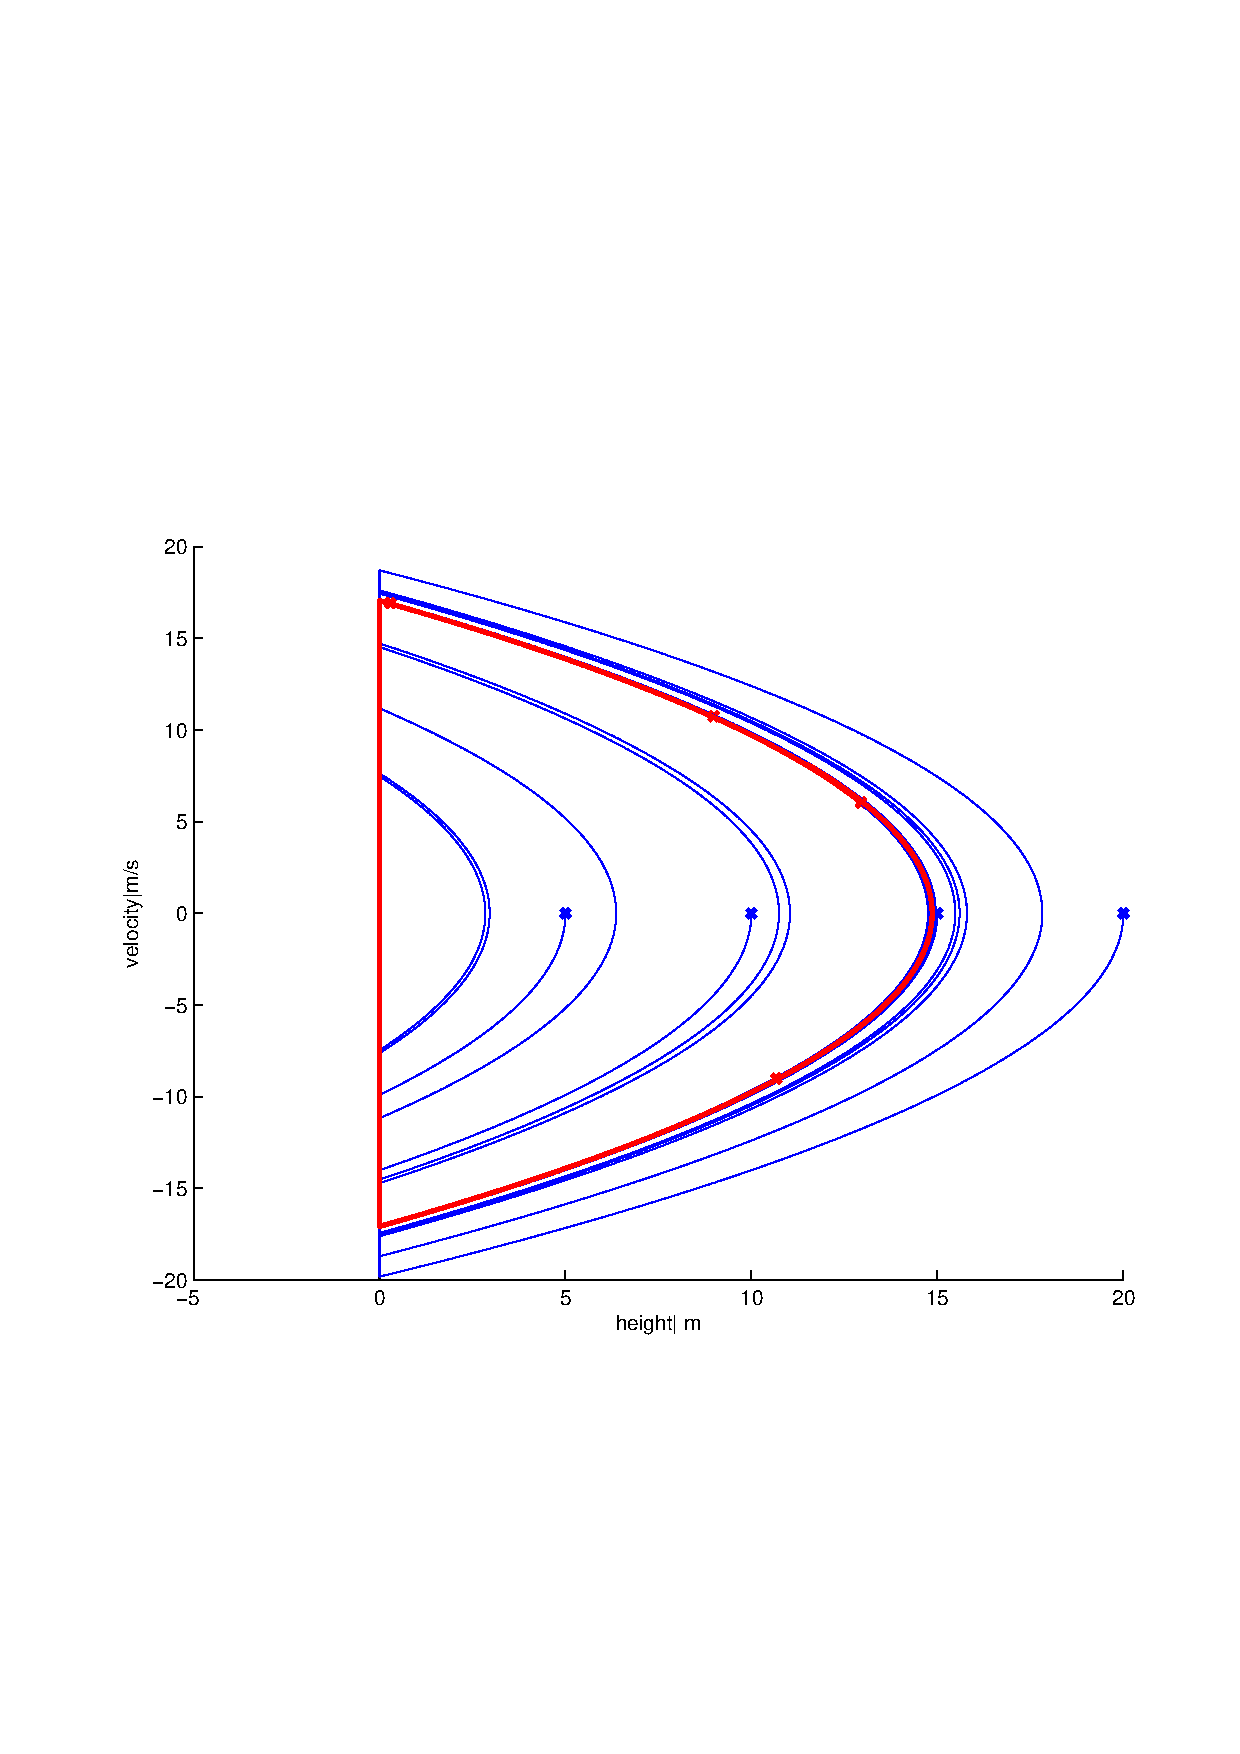
\includegraphics[width=0.7\textwidth]{BouncingBallPhasePlotAction3}
    \fi
    \caption{Energy Scaling}
    \label{fig:energy3}
  \end{center}
\end{figure}

\section{Combine Motion Primitives}

\subsection{The Motion Primitives Graph}
Motion Primitives comes from the original mechanical system, motion primitives can only transformed if they are neighbours.
Following this idea, given a dynamic system we can draw a graph of motion primitives and this is called motion primitives graph.
The idea is very similar to the motion graph, the difference here is in the original motion graph are handed  crafted, 
while in our research, we propose that a motion graph of a dynamic system is fixed, at from any motion primitives, the way he can change its motion is also limited.

\begin{figure}[!htbp]
  \begin{center}
    \leavevmode
    \ifpdf
      \includegraphics[height=6in]{MotionPrimitiveGraph}
    \else
      \includegraphics[width=0.7\textwidth]{MotionPrimitiveGraph}
    \fi
    \caption{Phase Plot of Motion Primitives}
    \label{fig:manyprimitives}
  \end{center}
\end{figure}


\begin{figure}[!htbp]
  \begin{center}
    \leavevmode
    \ifpdf
      \includegraphics[height=6in]{motiongraphtopology}
    \else
      \includegraphics[width=0.7\textwidth]{motiongraphtopology}
    \fi
    \caption{Phase Plot of Motion Primitives}
    \label{fig:manyprimitives}
  \end{center}
\end{figure}


\subsection{The Motion Primitives Transition}

From dynamic point of view, changing motion primitives is put the current state in the basin of attraction  of one attractor into the basic of attraction of another attractor.
As show in picture, for the uncontrolled system, the transition will not happen automatically, for the two basic of attraction will not overlap.

To put the state x in basin of attraction, have two methods.


\begin{figure}[!htbp]
  \begin{center}
    \leavevmode
    \ifpdf
      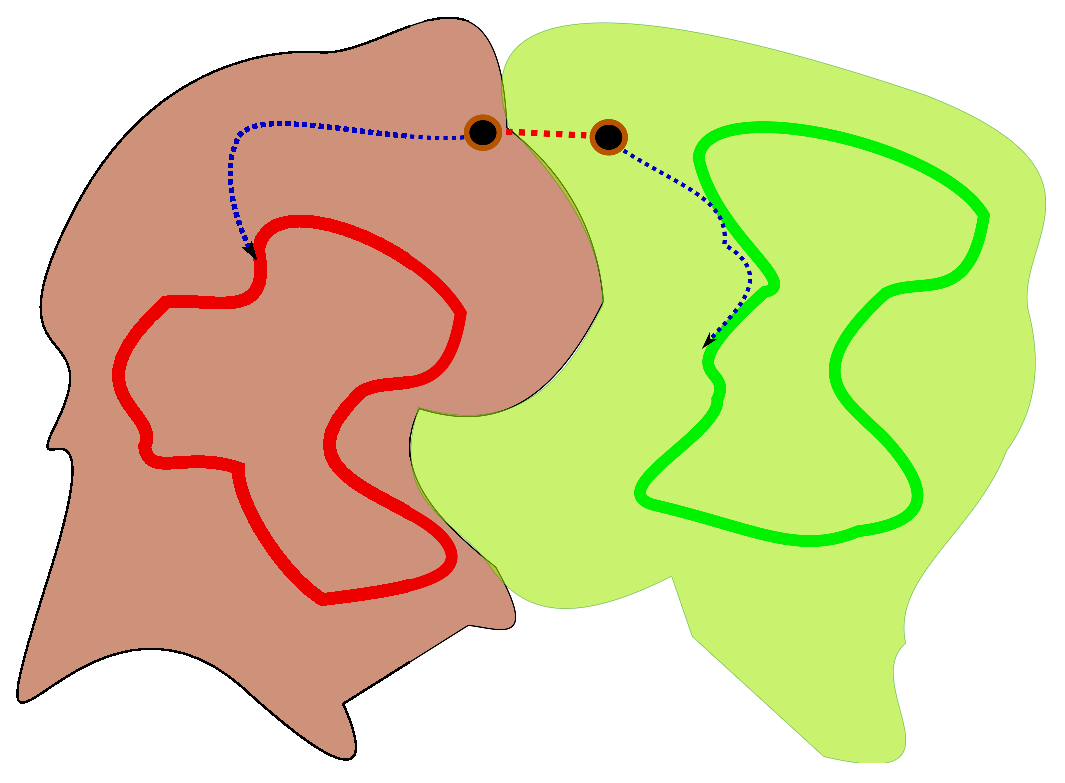
\includegraphics[height=6in]{MotionPrimitiveTransition}
    \else
      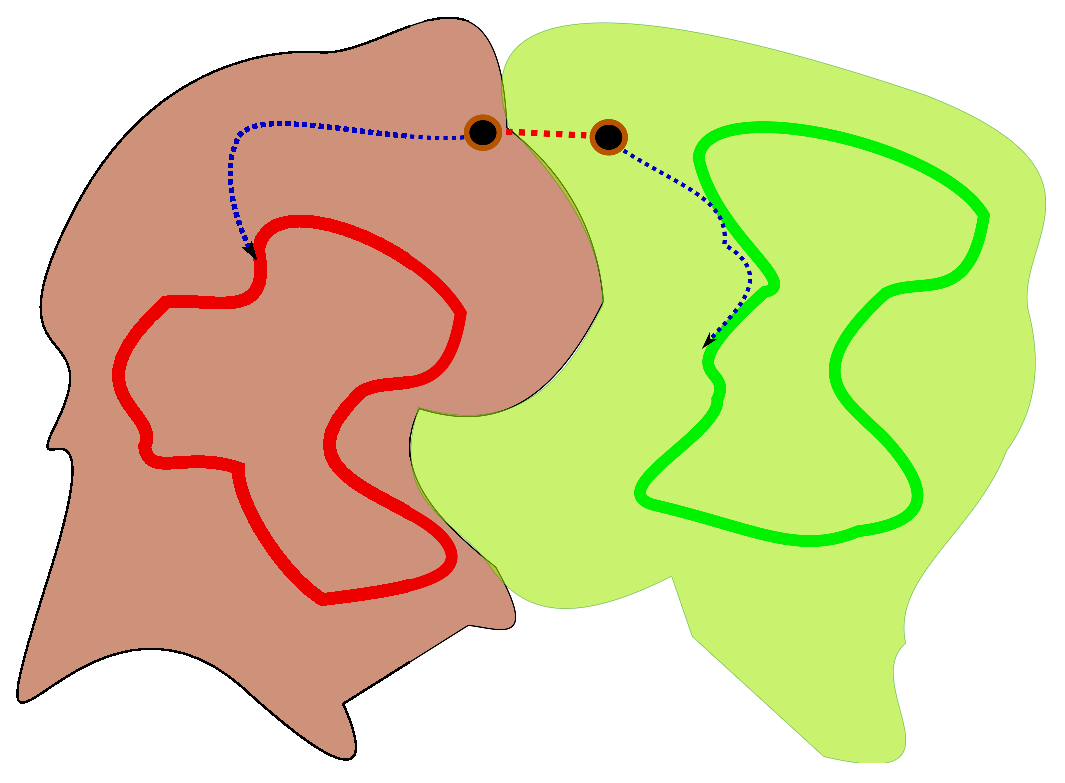
\includegraphics[width=0.7\textwidth]{MotionPrimitiveTransition}
    \fi
    \caption{Motion Primitive Transition}
    \label{fig:motion-transition}
  \end{center}
\end{figure}

\begin{itemize}
\HiItem{ Overlaping Method}
The first idea is use different CPG for different motion primitives. There is a switch mechanism of switching the CPG.
If cpa a is applied to the fx, then the basic off attraction is enlarged, if cpg b is applied to motion primitives b,
the basin of attraction is also enlarged.
If a system is at state that within the both basin of attraction, we can switch the CPG controller.

\begin{figure}[!htbp]
  \begin{center}
    \leavevmode
    \ifpdf
      \includegraphics[height=6in]{OverLayTransition}
    \else
      \includegraphics[width=0.7\textwidth]{OverLayTransition}
    \fi
    \caption{Over Lay Transition}
    \label{fig:motion-transition}
  \end{center}
\end{figure}


\HiItem{Transform Method}
Controlled Symmetr can also applied for motion state transition.
For a system at x , we can transform the phase portrait to make it which in the basic of attraction of b,
this is illustrate in figure 


\begin{figure}[!htbp]
  \begin{center}
    \leavevmode
    \ifpdf
      \includegraphics[height=6in]{OffsetTransition}
    \else
      \includegraphics[width=0.7\textwidth]{OffsetTransition}
    \fi
    \caption{Offset Transiton}
    \label{fig:transform-transit}
  \end{center}
\end{figure}
\end{itemize}




Both the method can result in physically realistic motion transition, when the current state x lies a a special position.
The what more problem happens when we don't know is where the current position x and where it is going.
Thus we combined the two method above to achieve for a combined method,
no matter where is current point is, it is going to converge to the limit cycle, thus we ask both basic of attraction cover the limit cycle, this can be achieved via using both the CPG and Transformation.
And for this usually ,both motion primitives needs to be transformed,
And the there is relationship between the two transformation,  this relation ship is called transformation connection.

Figure download show the illustrate the idea.

\begin{figure}[!htbp]
  \begin{center}
    \leavevmode
    \ifpdf
      \includegraphics[height=6in]{ConbineMethod}
    \else
      \includegraphics[width=0.7\textwidth]{ConbineMethod}
    \fi
    \caption{Comined Method}
    \label{fig:Combine}
  \end{center}
\end{figure}


